\section{Phosphorescence response characterization}
\label{appendix:phos:response}

Figures~\ref{fig:phos:resp:R01S00} through \ref{fig:phos:resp:R43S20} attempt to quantify the expressed phosphorescence response in ROIs on seven of the problematic ITL sensors. Previously, we had captured the phosphorescence {\it transient term} across the ITL sensors ({\it cf.} Figs.~\ref{fig:phos:R00} thru \ref{fig:phos:R44}); we also tracked ROI pixel distribution parameters of individual median images constructed from the selection of specific images acquired across the 20 B-protocol datasets available (listed in Table~\ref{tab:phosphorescence:datasets}). Here we analyze the signal level- and wavelength-dependences of the expressed phosphorescence captured in the first dark image following flat exposure. Table~\ref{tab:phos:sens:datasets} provides the dataset IDs and SeqIDs used for this analysis. 

\begin{center}
\begin{longtable}{lll}
\caption{Zephyr Scale E-numbers and corresponding SeqIDs analyzed to estimate signal level and wavelength dependence of the phosphorescence response.} \label{tab:phos:sens:datasets} \\
%\hline 
\toprule\noalign{}
%\multicolumn{1}{c}{\textbf{Run Type}} & 
\multicolumn{3}{c}{\textbf{Run numbers and SeqIDs of first dark following trigger}} \\
%\multicolumn{3}{c}{\textbf{(arranged by CCOB LED and trigger flat target signal)}} \\
%\multicolumn{1}{c}{\textbf{Third column}} \\ 
%\hline 
\midrule\noalign{}
\endfirsthead

\multicolumn{3}{c}%
{{\tablename\ \thetable{} -- continued from previous page}} \\
%\hline 
\toprule\noalign{}
%\multicolumn{1}{c}{\textbf{Run Type}} & 
\multicolumn{3}{c}{\textbf{Run numbers and SeqIDs of first dark following trigger}} \\
%\multicolumn{3}{c}{\textbf{(arranged by CCOB LED and trigger flat target signal)}} \\
%\hline 
\midrule\noalign{}
\endhead

%\hline 
\midrule\noalign{}
\multicolumn{3}{r}{{Continued on next page}} \\ 
%\hline
\bottomrule\noalign{}
\endfoot

\hline \hline
\endlastfoot
\midrule\noalign{}
CCOB LED & trigger flat target signal & runID \& SeqID \\
\midrule\noalign{}
uv &   500 & E1770:20241028\_000010 \\
uv &  1000 & E1503:20241020\_000489 \\
uv &  1500 & E1771:20241028\_000039 \\
uv &  3000 & E1504:20241020\_000533 \\
uv &  4500 & E1772:20241028\_000068 \\
uv &  5000 & E1505:20241020\_000577 \\
uv & 10000 & E1506:20241020\_000621 \\
uv & 13500 & E1773:20241028\_000097 \\
uv & 30000 & E1507:20241020\_000665 \\
\midrule\noalign{}
blue &   500 & E1774:20241028\_000126 \\
blue &  1000 & E1502:20241020\_000445 \\
blue &  1500 & E1775:20241028\_000155 \\
blue &  3000 & E1501:20241020\_000401 \\
blue &  4500 & E1776:20241028\_000184 \\
blue &  5000 & E1500:20241020\_000357 \\
blue & 10000 & E1499:20241020\_000313 \\
blue & 13500 & E1777:20241028\_000213 \\
blue & 30000 & E1498:20241020\_000269 \\
blue & 50000 & E1491:20241018\_000989 \\
blue &150000 & E1485:20241018\_000725 \\
blue &400000 & E1484:20241018\_000678 \\
\midrule\noalign{}
red & 50000 & E1490:20241018\_000945 \\
red &150000 & E1486:20241018\_000769 \\
red &400000 & E1483:20241018\_000634 \\
\midrule\noalign{}
nm750 & 50000 & E1492:20241018\_001033 \\
nm750 &150000 & E1487:20241018\_000813 \\
nm750 &400000 & E1479:20241018\_000543 \\
\midrule\noalign{}
nm850 & 50000 & E1493:20241018\_001077 \\
nm850 &150000 & E1488:20241018\_000857 \\
nm850 &400000 & E1477:20241018\_000455 \\
\midrule\noalign{}
nm960 & 50000 & E1494:20241018\_001121 \\
nm960 &150000 & E1489:20241018\_000901 \\
nm960 &400000 & E1478:20241018\_000499 \\
\bottomrule\noalign{}
\end{longtable}
\end{center}


These runs were performed to sample a two-dimensional, rectangular parameter space, and each measurement was executed only once. The resulting sampling was completed incrementally, over 3 separate days. Using only one image for each data point, we were not able to median multiple images acquired under identical conditions (as we had done for Sections~\ref{appendix:phos:ident}, \ref{appendix:phos:coffeestains} and \ref{appendix:phos:kinetics}). 

Because there is significant variation in morphological characteristics of the phosphorescence, we adopted the following strategy to quantify phosphorescence expression in each: Once the image is processed through ISR, each of the sensor specific ROIs are used to filter the pixels, and the signal distribution parameters are evaluated. The 99\% quantile signal level was used as a bright end proxy for the expressed phosphorescence for each ROI. A consequence of this is that when there is insignificant or undetectable phosphorescence, this proxy choice would be artificially high, which would be pegged at about 4$\sigma$ above the noise distribution mean. 

The figures provide dashed lines that represent constant {\it phosphorescence efficiency ratios} to guide the eye (at 10\%, 1\% and 0.1\%), while different color LED illumination are represented by different plotting symbols and line colors. The only CCOB LED used across the entire range of trigger flat signal levels is the {\it blue} one. The 400k$e^-$ {\it blue} LED trigger flat induced phosphorescence levels are the only ones described thus far in Sections~\ref{appendix:phos:ident}, \ref{appendix:phos:coffeestains} and \ref{appendix:phos:kinetics}.  

Two of the sensors exhibiting distributed and structured phosphorescence expression (R02\_S02 \& R43\_S20) appear to have phosphorescence yields below $3\times 10^{-3}$ for {\it uv} and {\it blue} LED illumination. Given the kinetics studied for these ROIs for {\it blue} LED illumination ({\it cf.} Figs~\ref{fig:phos:kinetics:R02S02} and \ref{fig:phos:kinetics:R43S20}), the worst case contribution may be 55~$e^-$/pix/15s ({\it uv} LED, $30{\mathrm k}e^{-} \times e^{+0.62} \times 10^{-3}$). The $e^{+0.62}$ scaling factor comes from the fact that the LED flash occurs (and ends) at the beginning of the trigger flat illumination and typically lasts for just a fraction of the image time of $\sim17.5$ seconds.

One other sensor with distributed, coffee stain-like phosphorescence (R02\_S12) shows significantly more signal in one of the ROIs ({\it uv} and {\it blue} LEDs for 30k$e^-$ and 400k$e^-$, respectively). Upon applying the $e^{+0.62}$ factor, the worst case phosphorescence here would scale to 560$e^-$/pix/15s and 1800$e^-$/pix/15s, respectively.

The remaining four sensors (R01\_S00, R03\_S10, R20\_S20 \& R43\_S11) show even more phosphorescence. The first three of these are due to {\it vampire pixels} (with or without central hot spots), while the last one showed the diffuse glow along the edges which ``shuts off'' with HV Bias. The phosphorescent yield high-end proxy limits for these ROIs fall within the $10^{-2}$ to $10^{-1}$ range. There are even a few data points that approach or exceed $10^{-1}$ (R03\_S10 \& R20\_S20) and such phosphorescence levels might be hard to believe, especially if the LED flash timing correction factor of $e^{+0.62}$ is also applied. One thing to keep in mind is that {\it vampire pixels} are known to bend drift field lines to produce regions with (apparently) $>100\%$ QE. For example, the {\it vampire pixel} on R03\_S10\_C15 contains a group of pixels that can receive up to 15$\times$ the target level in a flat exposure, so such large yields as we've seen here are perhaps not so mysterious after all.

\begin{figure}[!htbp]
\centering
\begin{subfigure}{0.45\textwidth}    
  \centering
  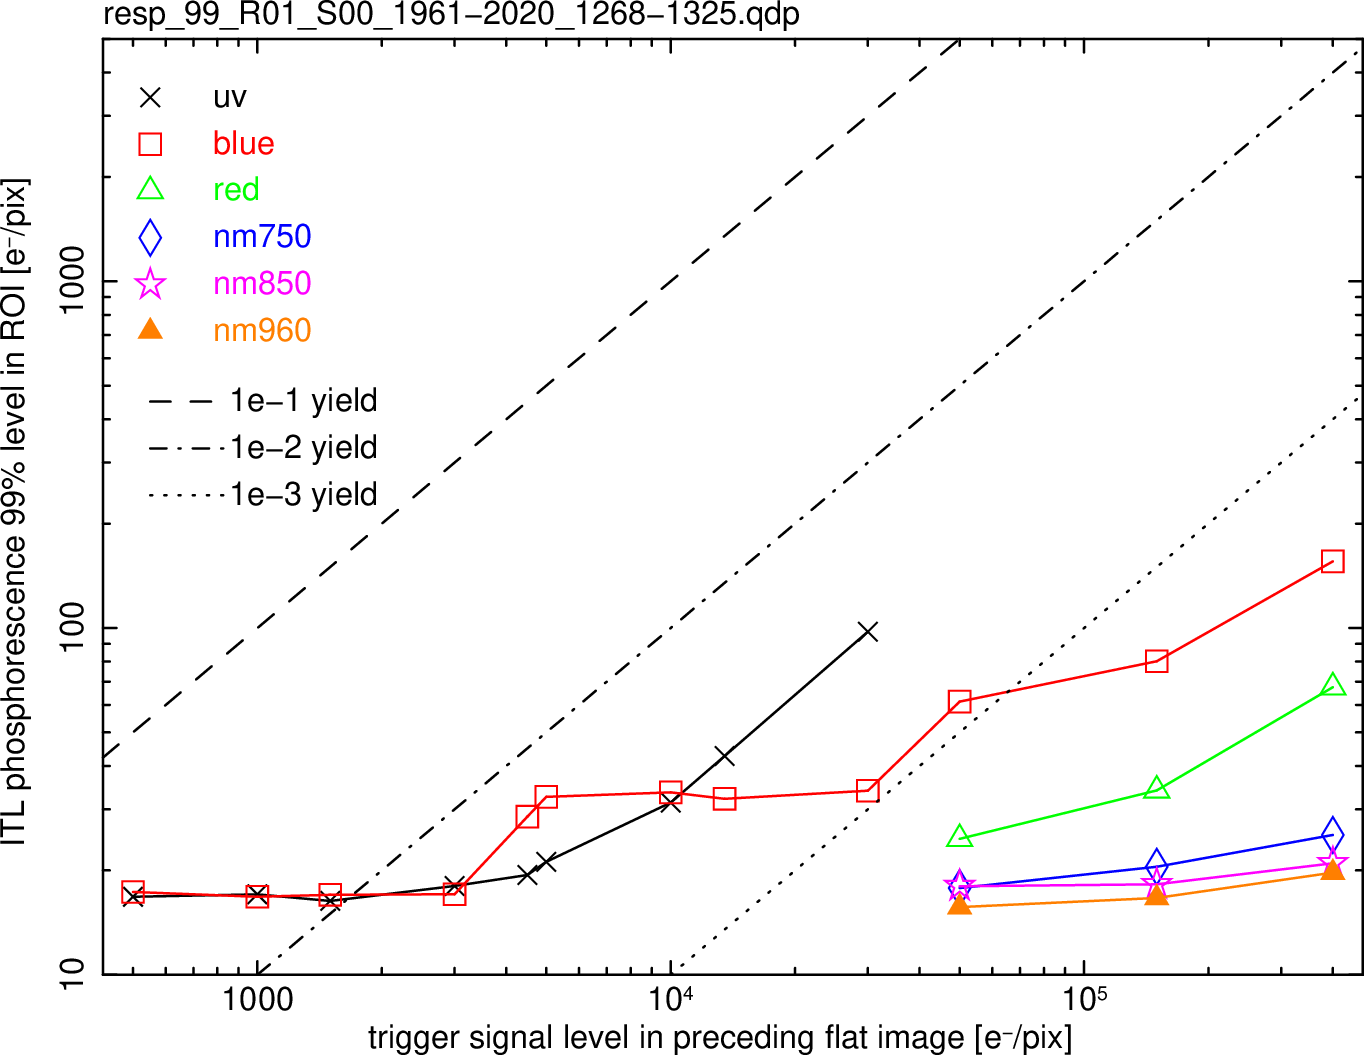
\includegraphics[width=\textwidth]{figures/phosphorescence-survey/phos_resp/resp_99_R01_S00_1961-2020_1268-1325.png}    
\end{subfigure}
\newline
\centering
\begin{subfigure}{0.45\textwidth}    
  \centering
  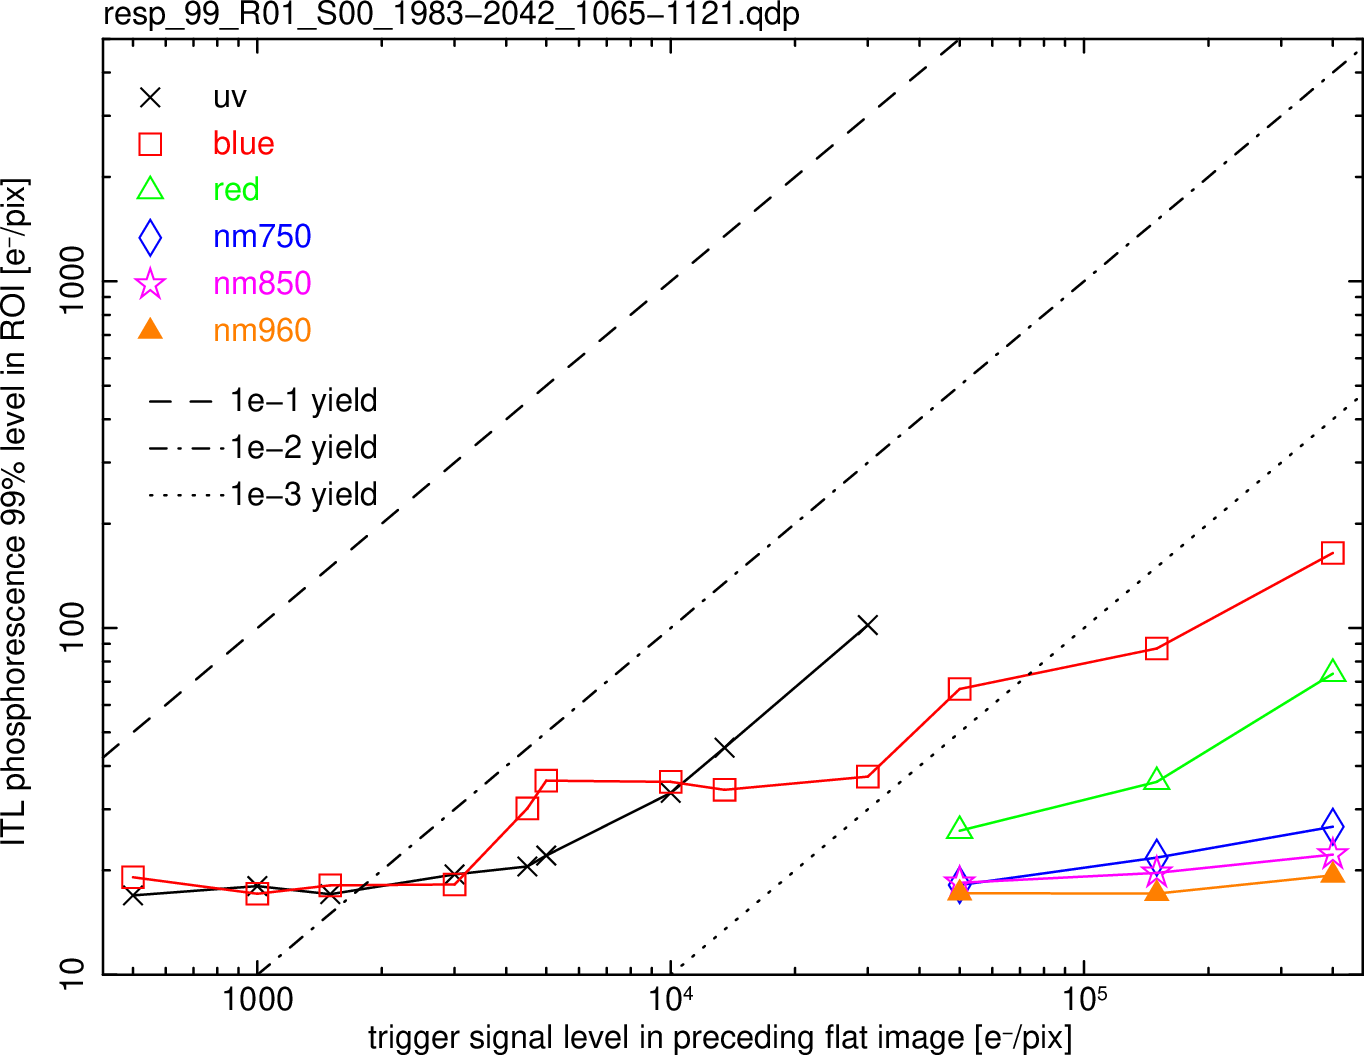
\includegraphics[width=\textwidth]{figures/phosphorescence-survey/phos_resp/resp_99_R01_S00_1983-2042_1065-1121.png}    
\end{subfigure}
\newline
\centering
\begin{subfigure}{0.45\textwidth}    
  \centering
  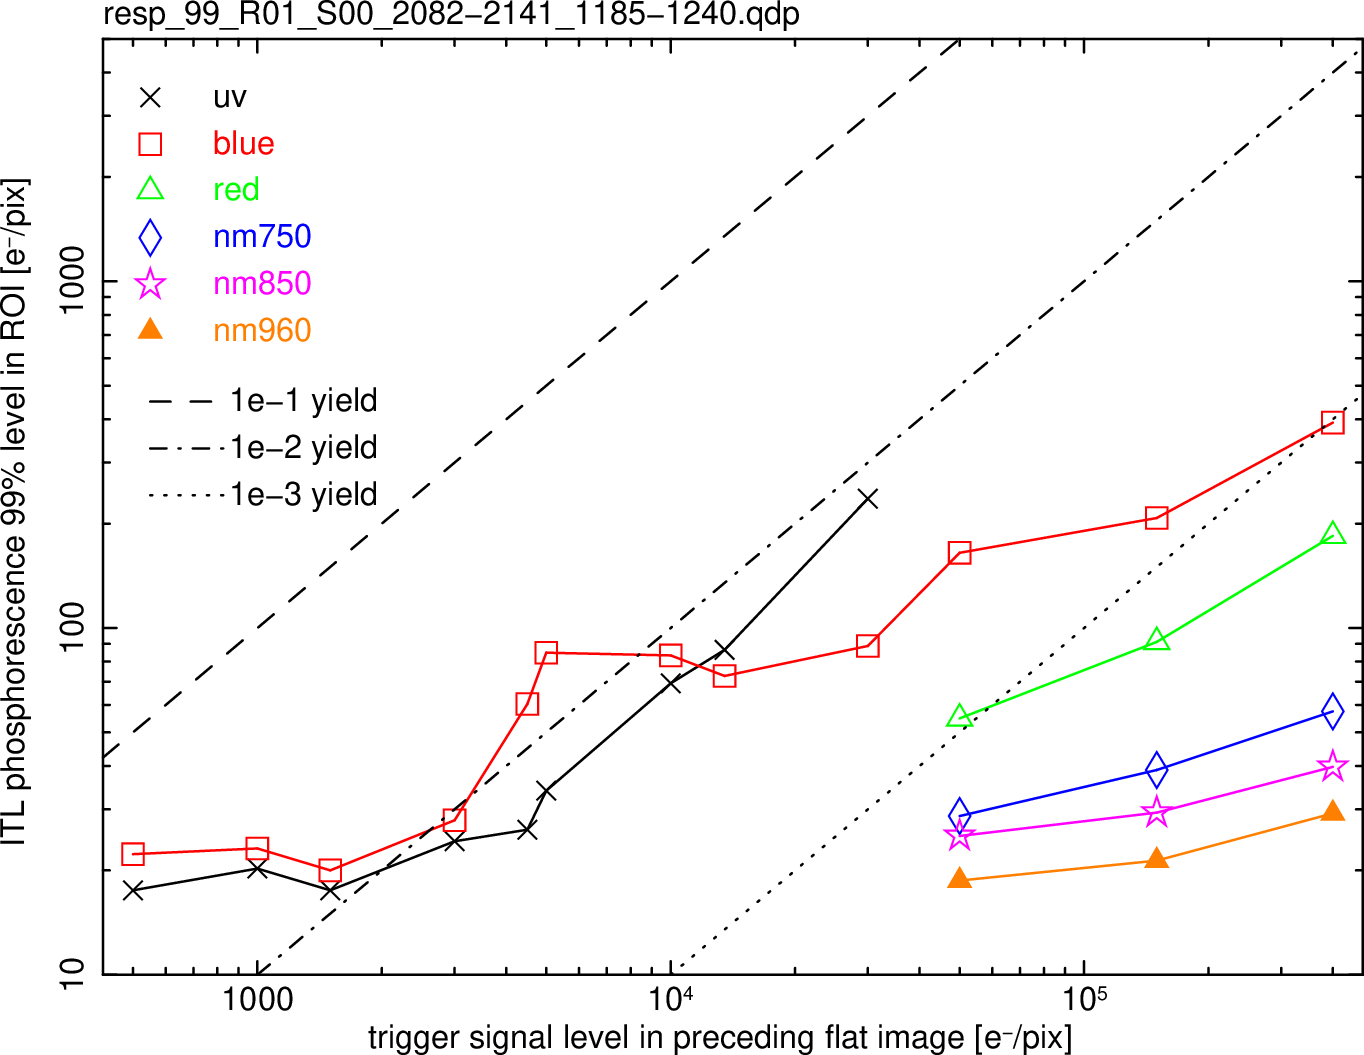
\includegraphics[width=\textwidth]{figures/phosphorescence-survey/phos_resp/resp_99_R01_S00_2082-2141_1185-1240.png}    
\end{subfigure}
\newline
\caption{Signal and wavelength response for phosphorescence expression (99\% level) in ROIs of images for R01\_S00. This is the prominent cosmetic seen in Fig.~\ref{fig:phos:stains:R01S00}, which is apparently a {\it vampire} pixel.}
\label{fig:phos:resp:R01S00}
\end{figure}

\begin{figure}[!htbp]
\centering
\begin{subfigure}{0.45\textwidth}    
  \centering
  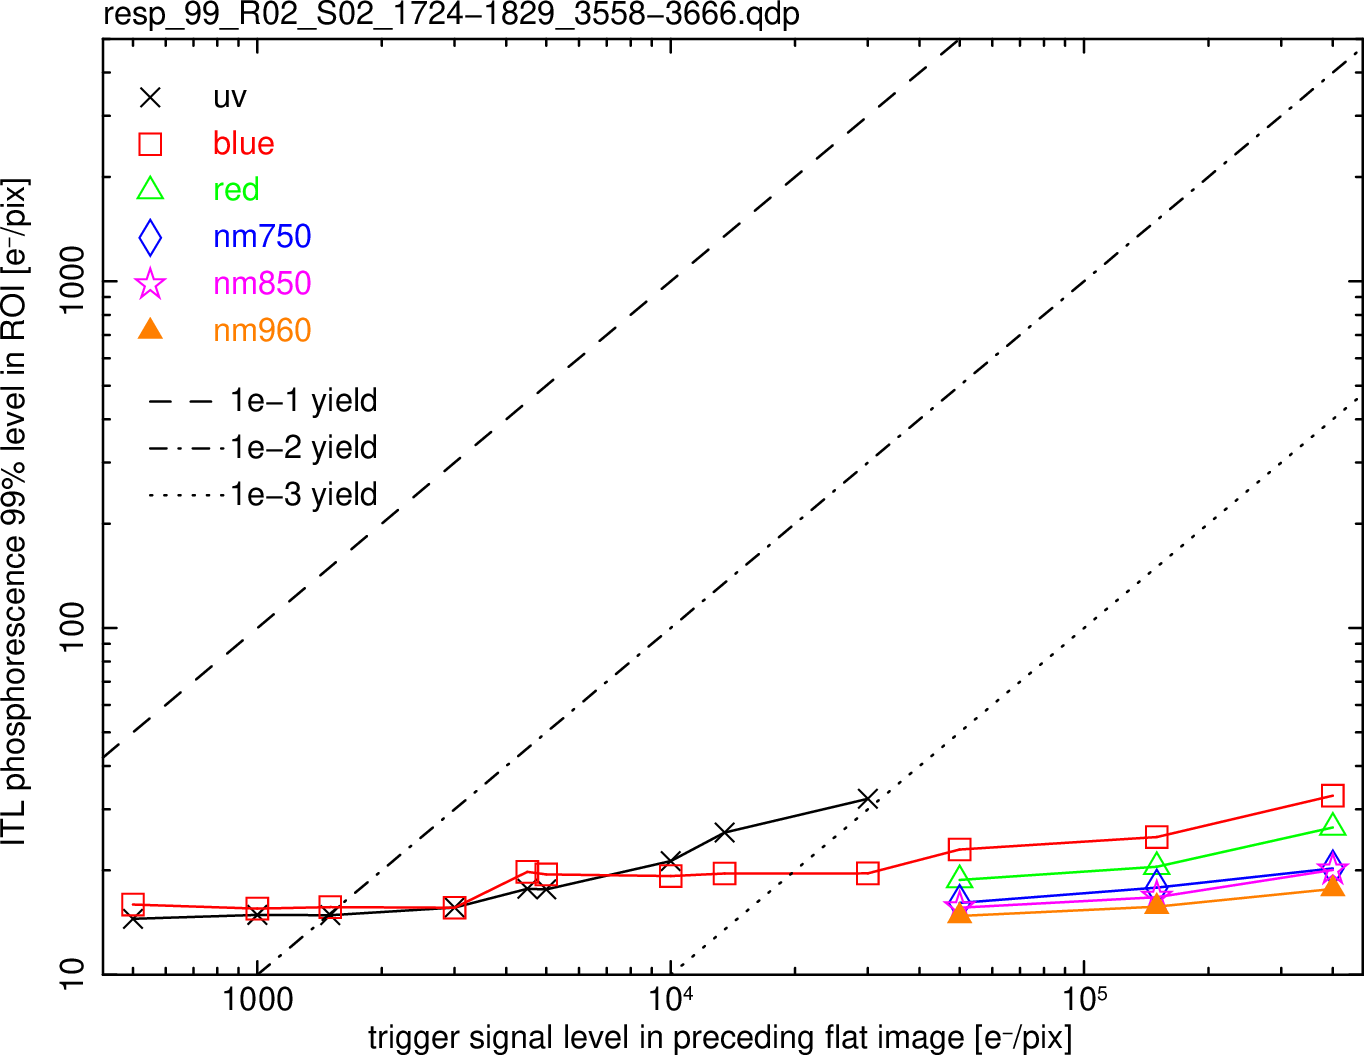
\includegraphics[width=\textwidth]{figures/phosphorescence-survey/phos_resp/resp_99_R02_S02_1724-1829_3558-3666.png}    
\end{subfigure}
\newline
\centering
\begin{subfigure}{0.45\textwidth}    
  \centering
  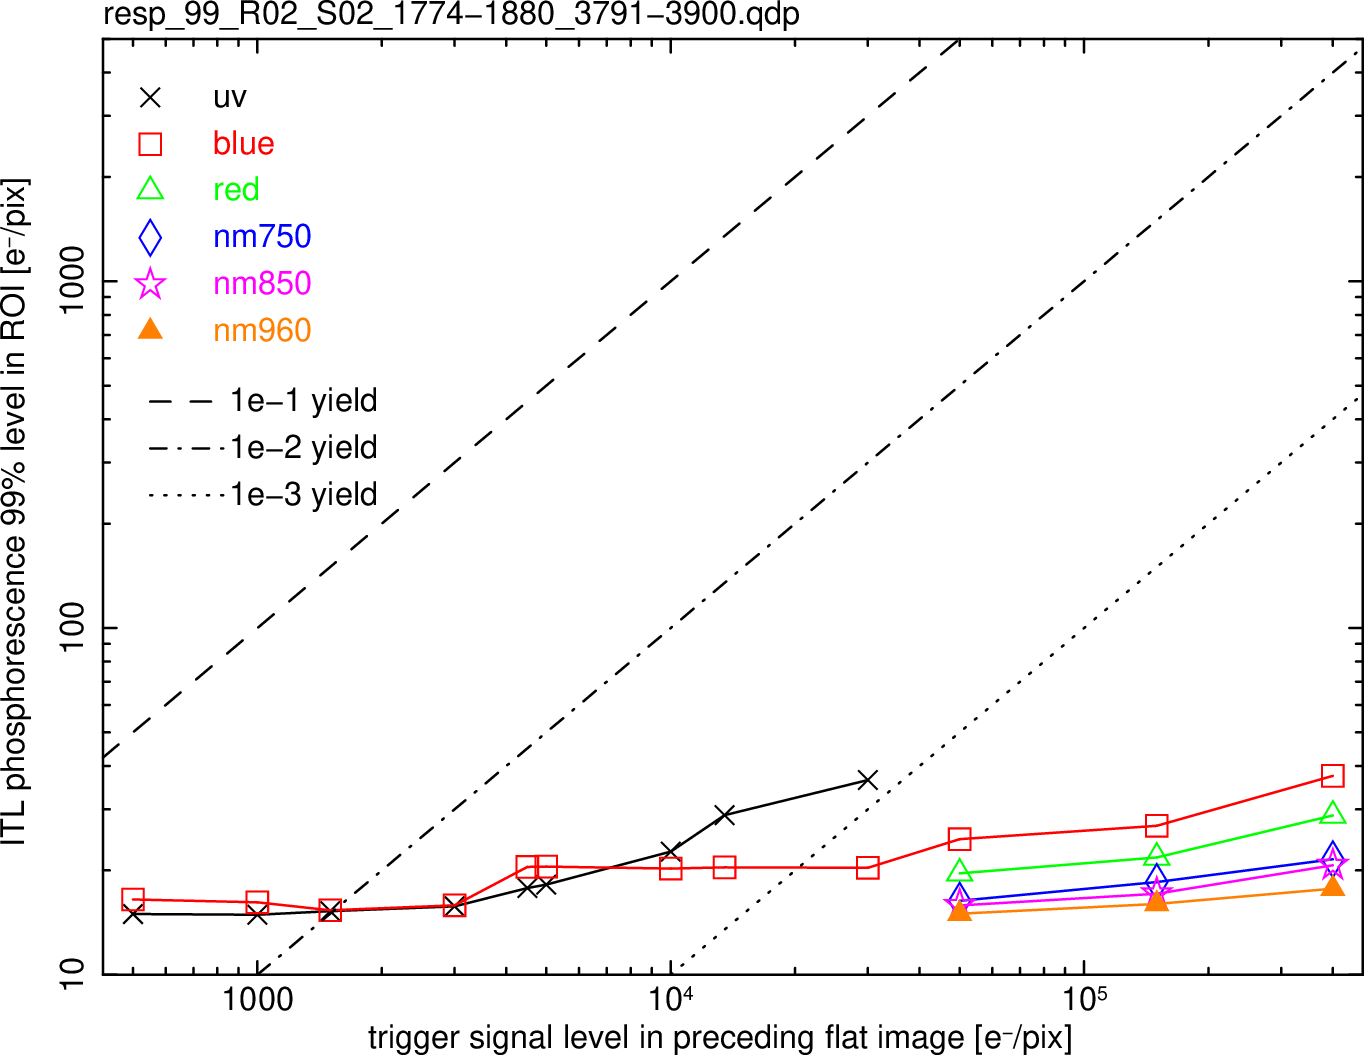
\includegraphics[width=\textwidth]{figures/phosphorescence-survey/phos_resp/resp_99_R02_S02_1774-1880_3791-3900.png}    
\end{subfigure}
\newline
\centering
\begin{subfigure}{0.45\textwidth}    
  \centering
  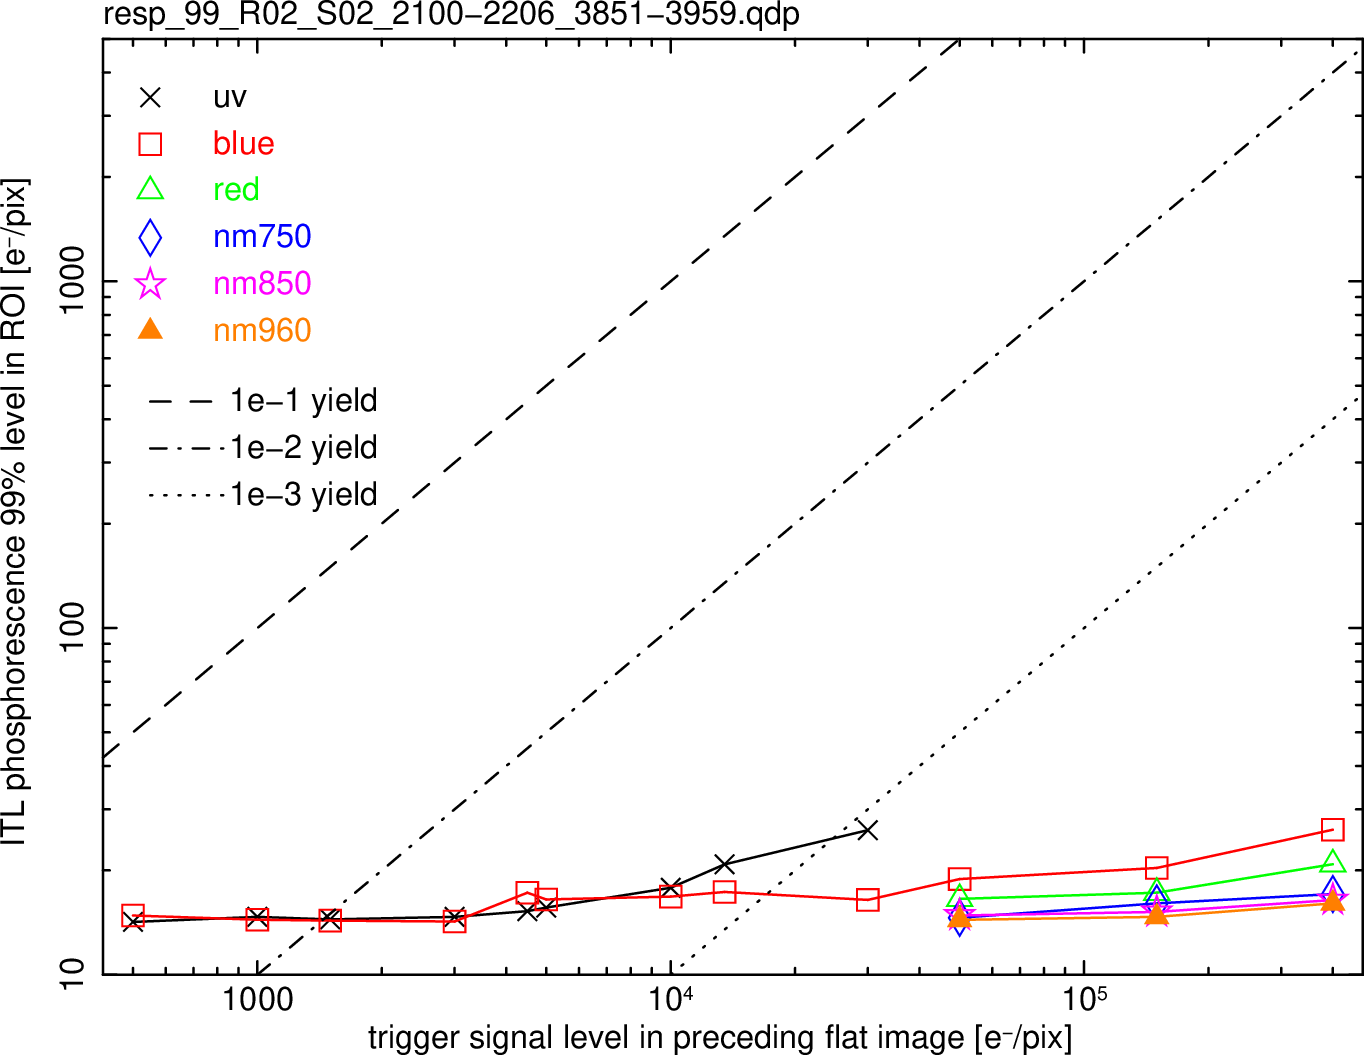
\includegraphics[width=\textwidth]{figures/phosphorescence-survey/phos_resp/resp_99_R02_S02_2100-2206_3851-3959.png}    
\end{subfigure}
\newline
\caption{Signal and wavelength response for phosphorescence expression (99\% level) in ROIs of images for R02\_S02. This is the diffuse phosphorescence that correlates with the coffee stains seen in Fig.~\ref{fig:phos:stains:R02S02}. No extractions were performed on the {\it vampire pixels} found on the same sensor (R02\_S02\_C15 and R02\_S02\_C07).}
\label{fig:phos:resp:R02S02}
\end{figure}

\begin{figure}[!htbp]
\centering
\begin{subfigure}{0.45\textwidth}    
  \centering
  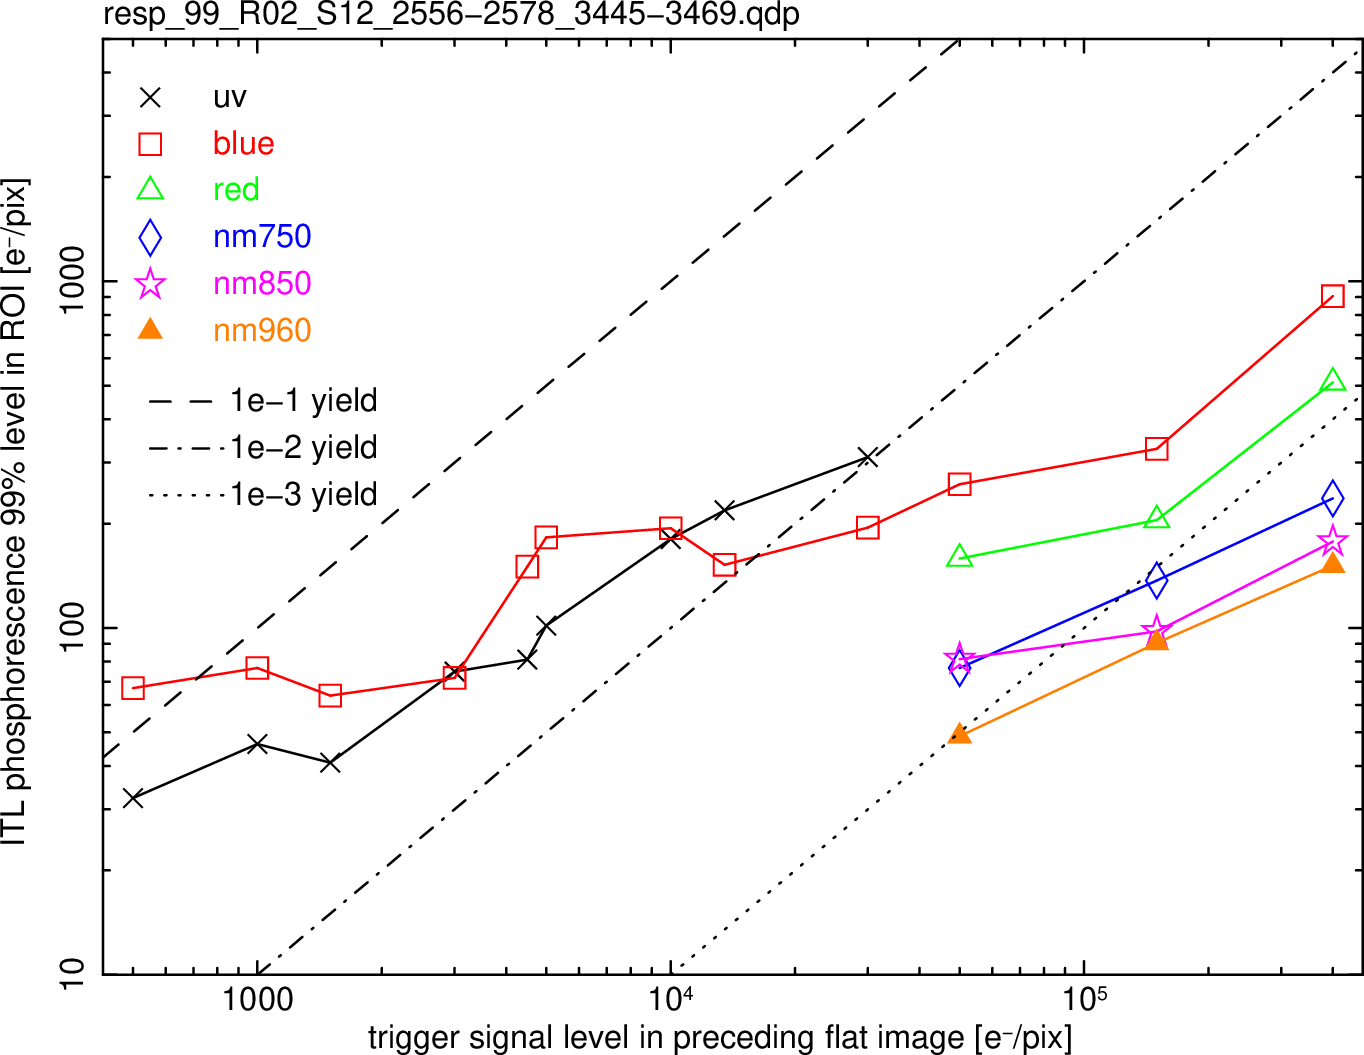
\includegraphics[width=\textwidth]{figures/phosphorescence-survey/phos_resp/resp_99_R02_S12_2556-2578_3445-3469.png}    
\end{subfigure}
\newline
\centering
\begin{subfigure}{0.45\textwidth}    
  \centering
  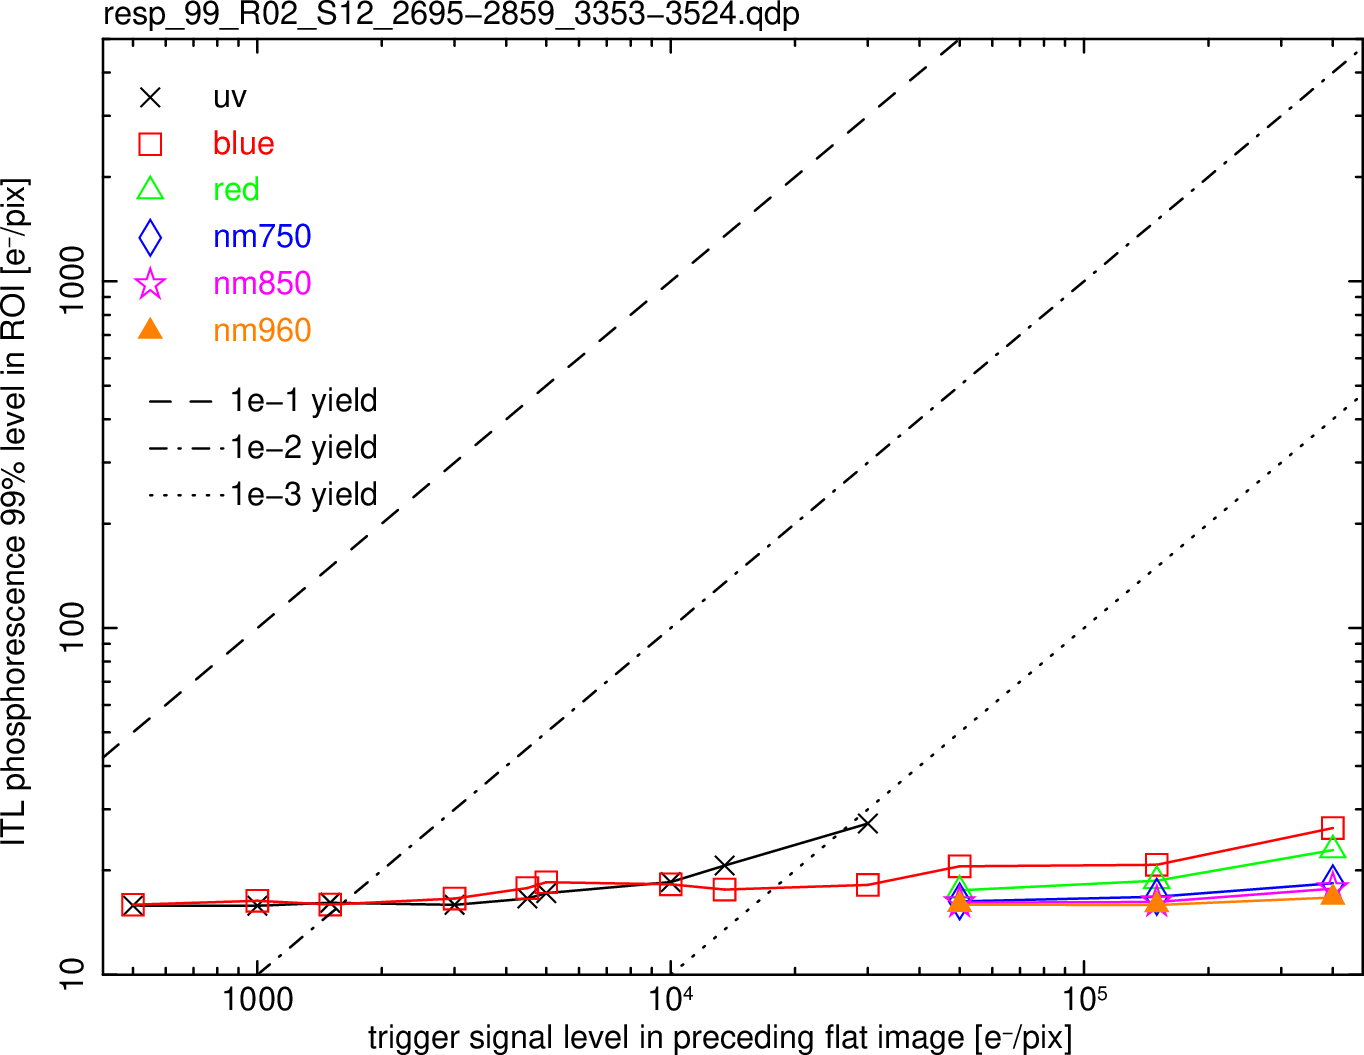
\includegraphics[width=\textwidth]{figures/phosphorescence-survey/phos_resp/resp_99_R02_S12_2695-2859_3353-3524.png}    
\end{subfigure}
\newline
\centering
\begin{subfigure}{0.45\textwidth}    
  \centering
  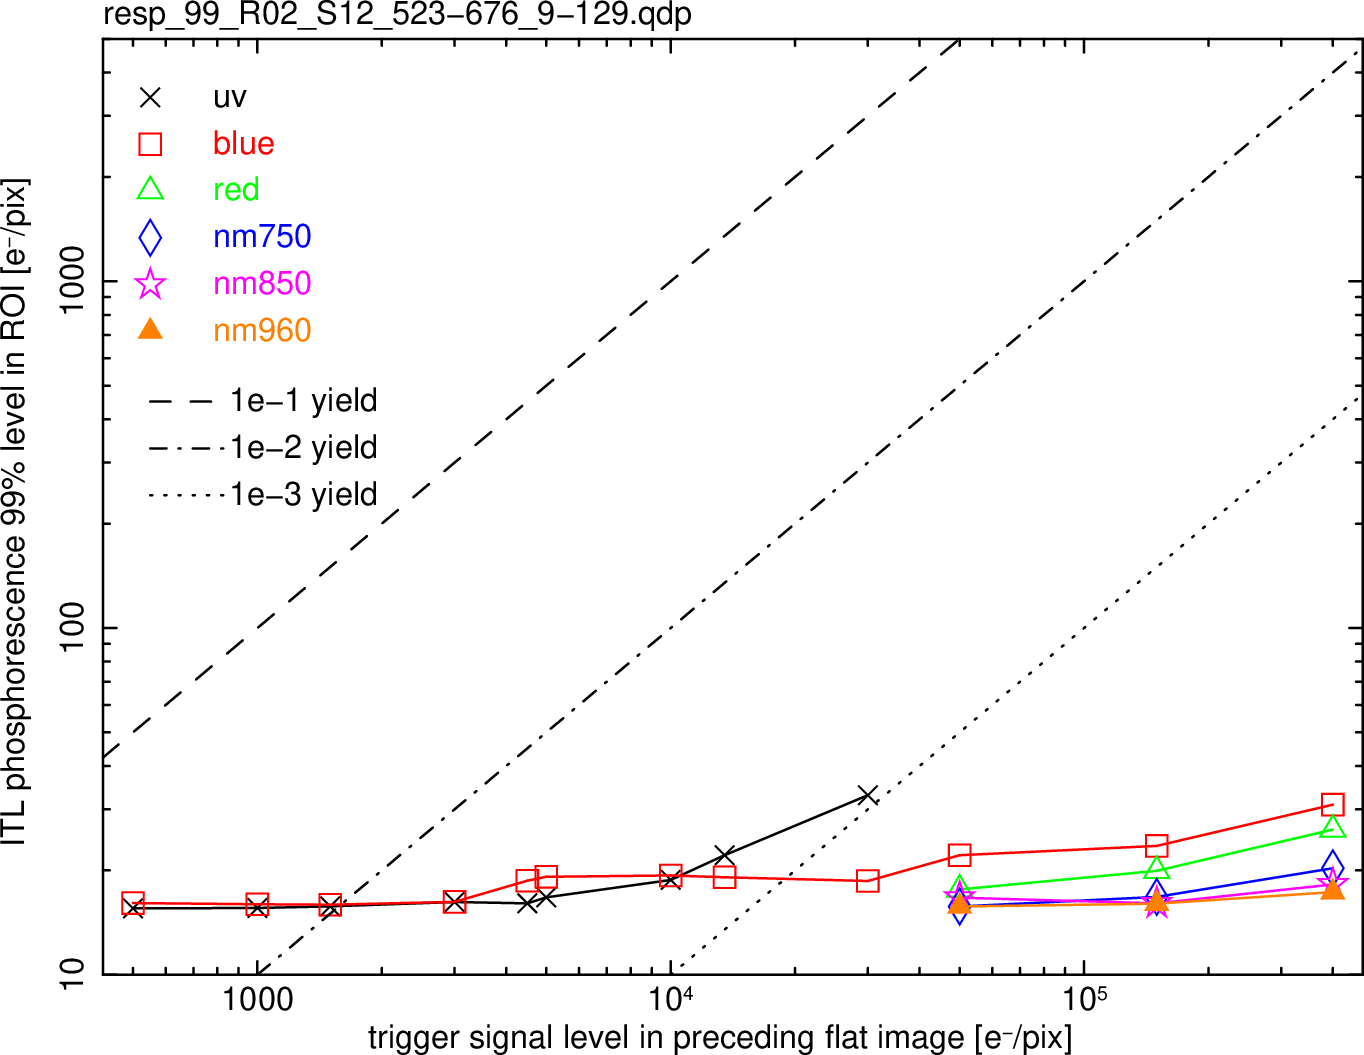
\includegraphics[width=\textwidth]{figures/phosphorescence-survey/phos_resp/resp_99_R02_S12_523-676_9-129.png}    
\end{subfigure}
\newline
\caption{Signal and wavelength response for phosphorescence expression (99\% level) in ROIs of images for R02\_S12. This is the structured phosphorescence that correlates with the coffee stains seen in Fig.~\ref{fig:phos:stains:R02S12}.}
\label{fig:phos:resp:R02S12}
\end{figure}

\begin{figure}[!htbp]
\centering
\begin{subfigure}{0.45\textwidth}    
  \centering
  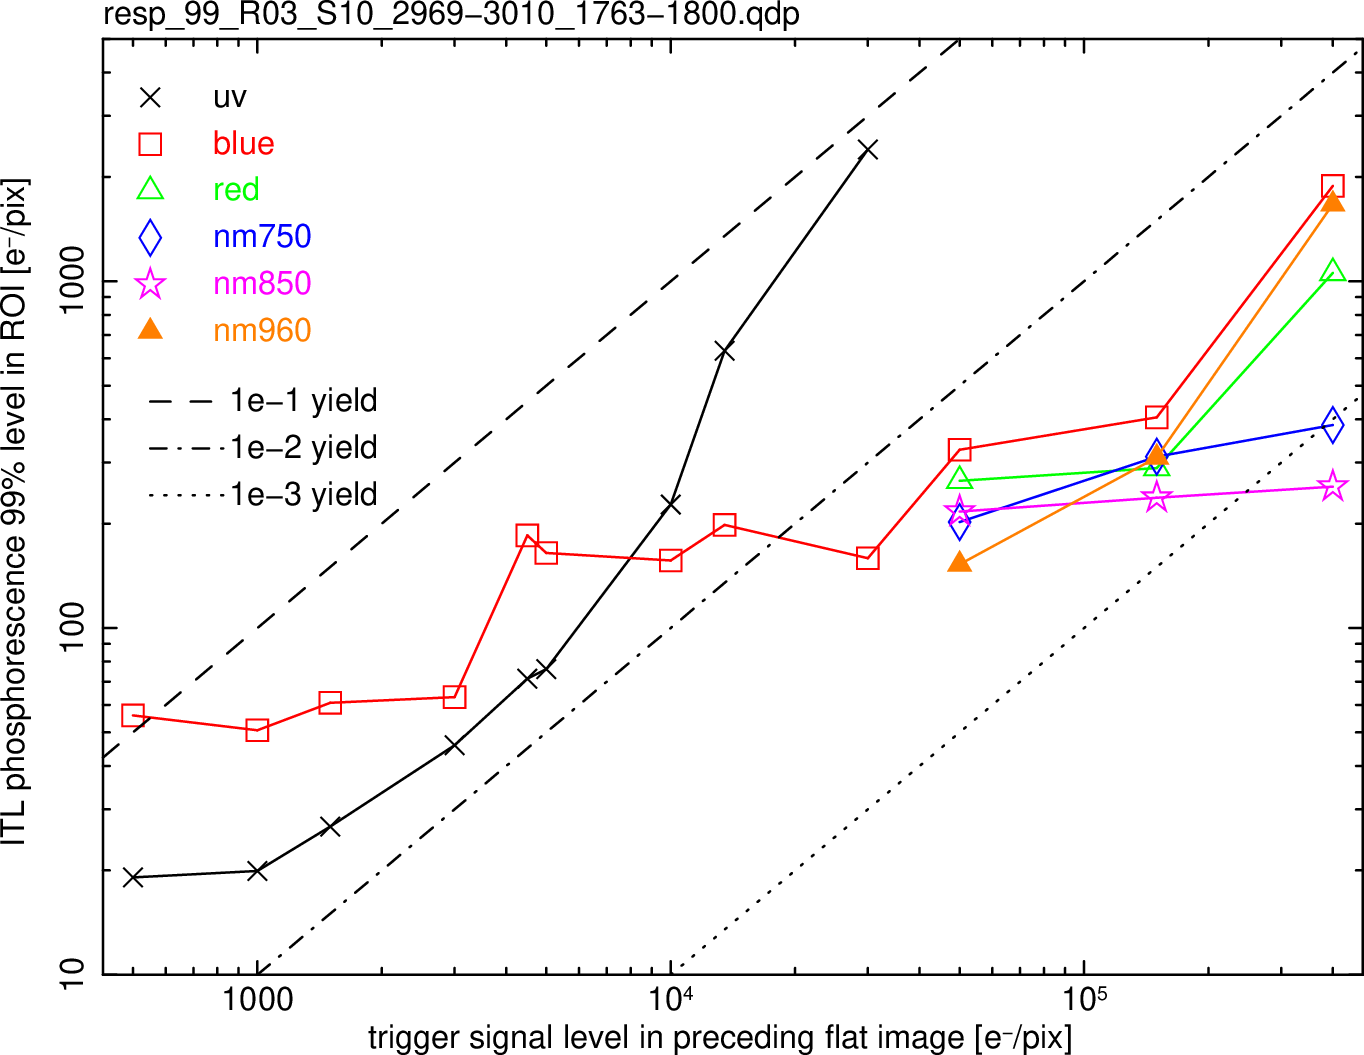
\includegraphics[width=\textwidth]{figures/phosphorescence-survey/phos_resp/resp_99_R03_S10_2969-3010_1763-1800.png}    
\end{subfigure}
\newline
\centering
\begin{subfigure}{0.45\textwidth}    
  \centering
  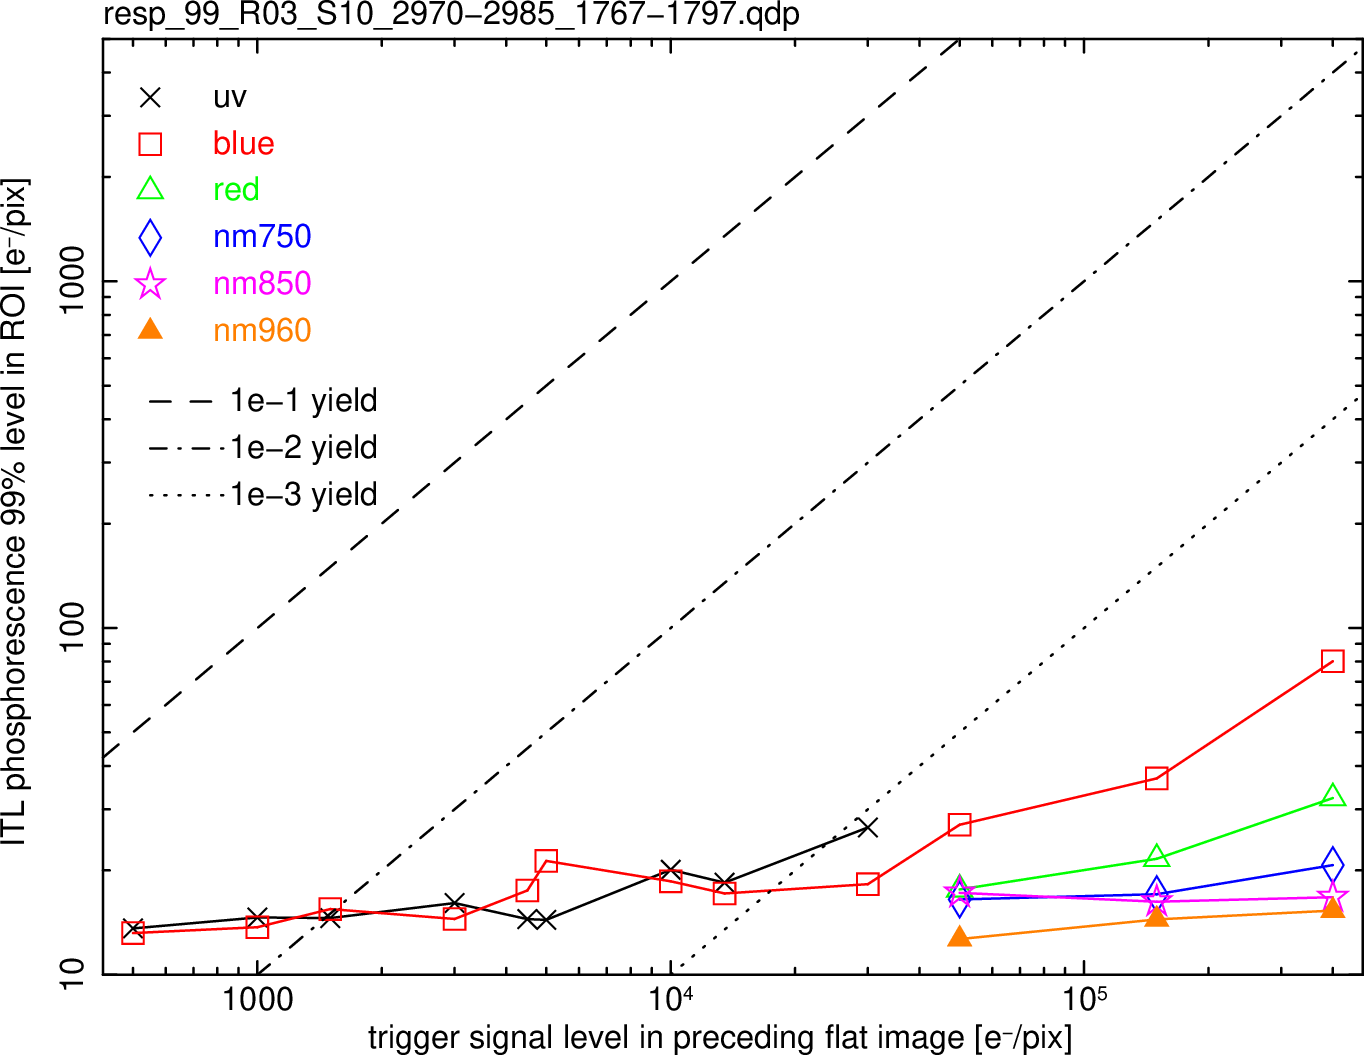
\includegraphics[width=\textwidth]{figures/phosphorescence-survey/phos_resp/resp_99_R03_S10_2970-2985_1767-1797.png}    
\end{subfigure}
\newline
\centering
\begin{subfigure}{0.45\textwidth}    
  \centering
  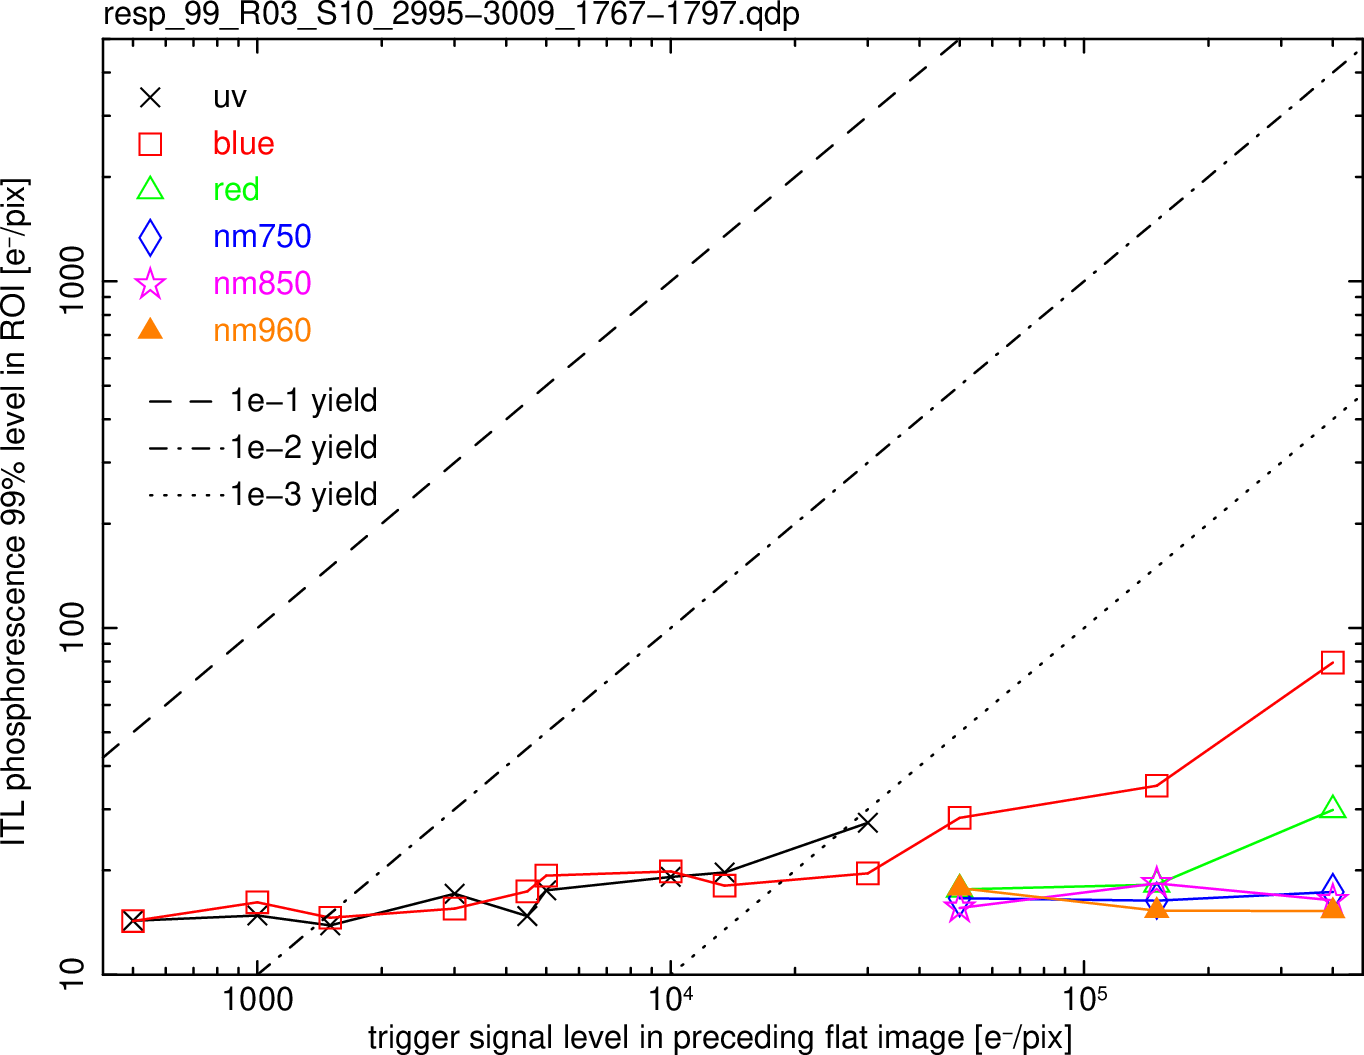
\includegraphics[width=\textwidth]{figures/phosphorescence-survey/phos_resp/resp_99_R03_S10_2995-3009_1767-1797.png}    
\end{subfigure}
\newline
\caption{Signal and wavelength response for phosphorescence expression (99\% level) in ROIs of images for R03\_S10. These describe regions including or near the bright/focusing {\it vampire pixel} seen in Figs.~\ref{fig:phos:stains:R03S10}, \ref{subfig:phosresp_R03_S10} and \ref{subfig:hvb_on_R03_S10}.}
\label{fig:phos:resp:R03S10}
\end{figure}

\begin{figure}[!htbp]
\centering
\begin{subfigure}{0.45\textwidth}    
  \centering
  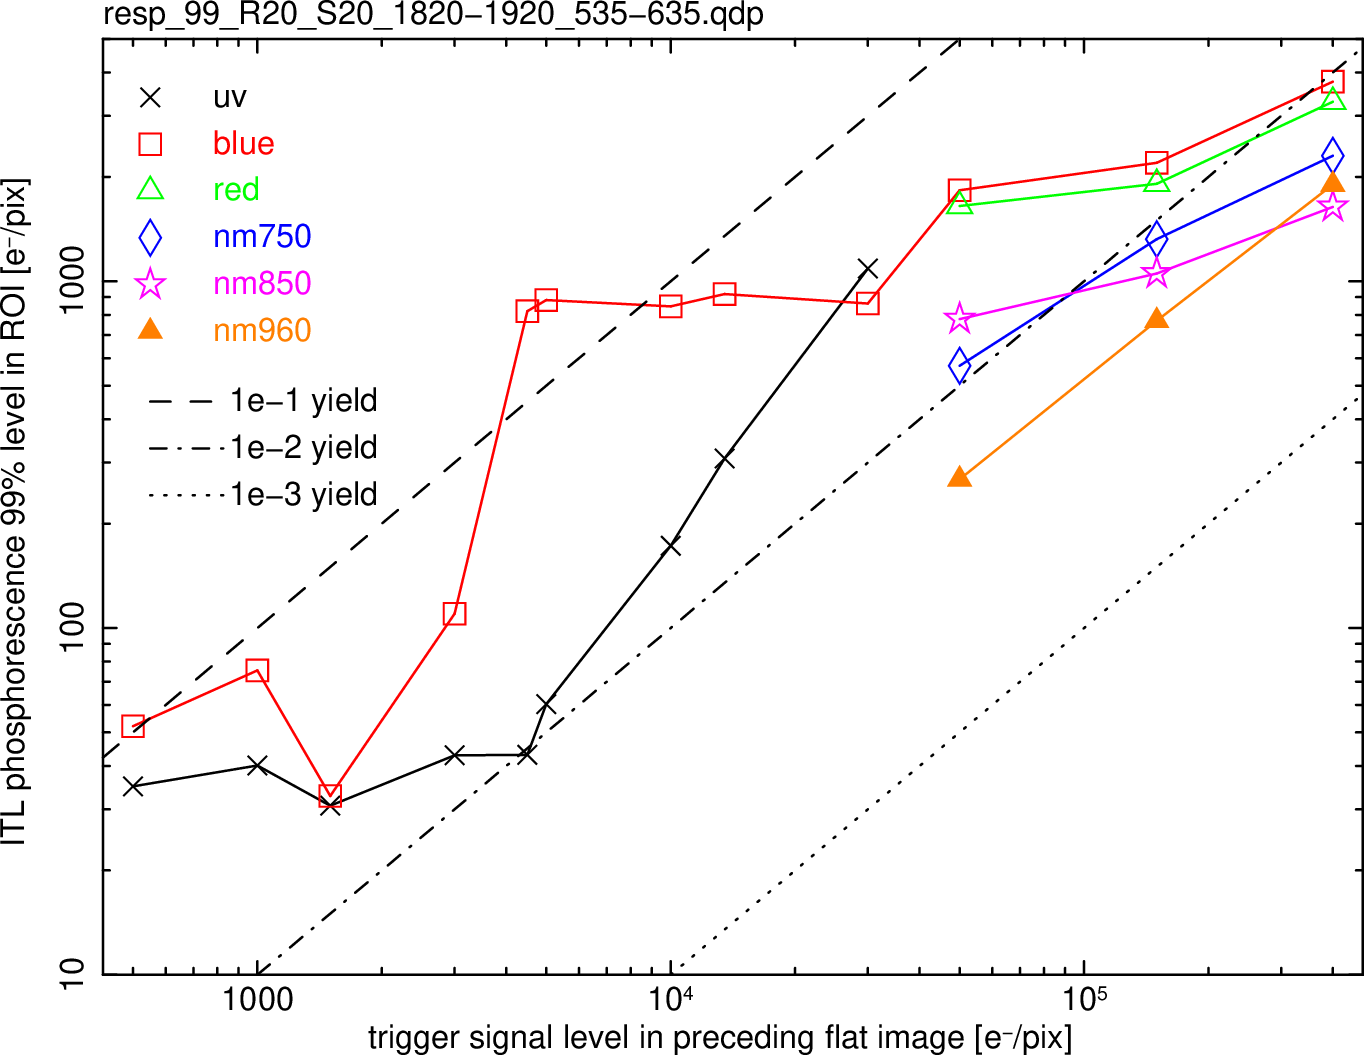
\includegraphics[width=\textwidth]{figures/phosphorescence-survey/phos_resp/resp_99_R20_S20_1820-1920_535-635.png}    
\end{subfigure}
\newline
\caption{Signal and wavelength response for phosphorescence expression (99\% level) in an ROI of images for R20\_S20. These describe the prominent non-focusing {\it vampire pixel} seen in Figs.~\ref{subfig:phosresp_R20_S20} and \ref{subfig:hvb_on_R20_S20}.}
\label{fig:phos:kinetics:R20S20}
\end{figure}

\begin{figure}[!htbp]
\centering
\begin{subfigure}{0.45\textwidth}    
  \centering
  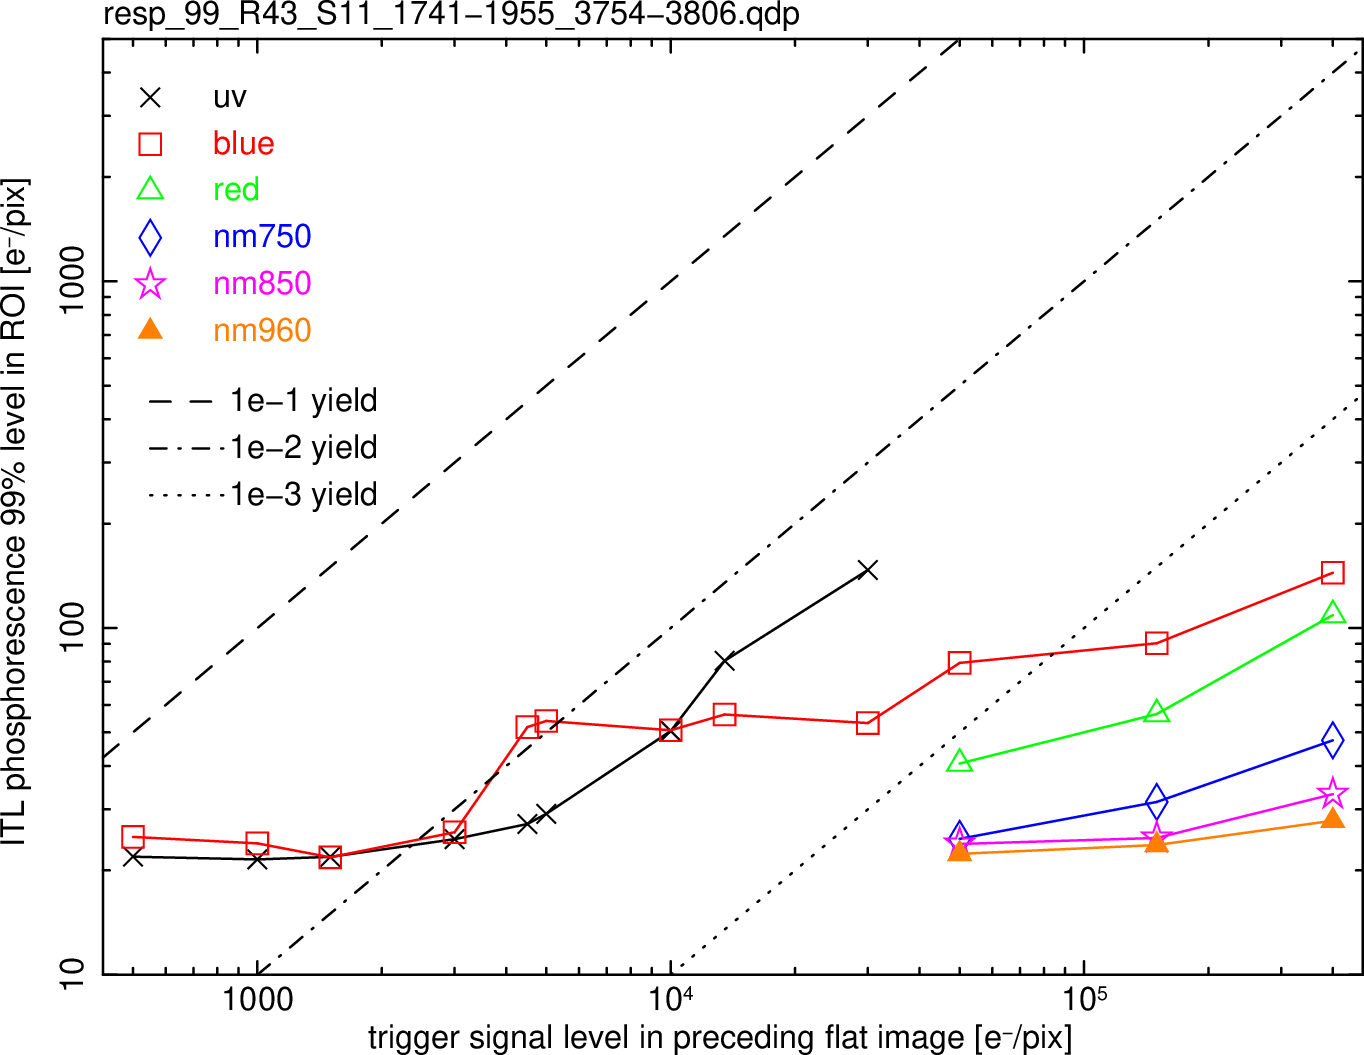
\includegraphics[width=\textwidth]{figures/phosphorescence-survey/phos_resp/resp_99_R43_S11_1741-1955_3754-3806.png}    
\end{subfigure}
\newline
\centering
\begin{subfigure}{0.45\textwidth}    
  \centering
  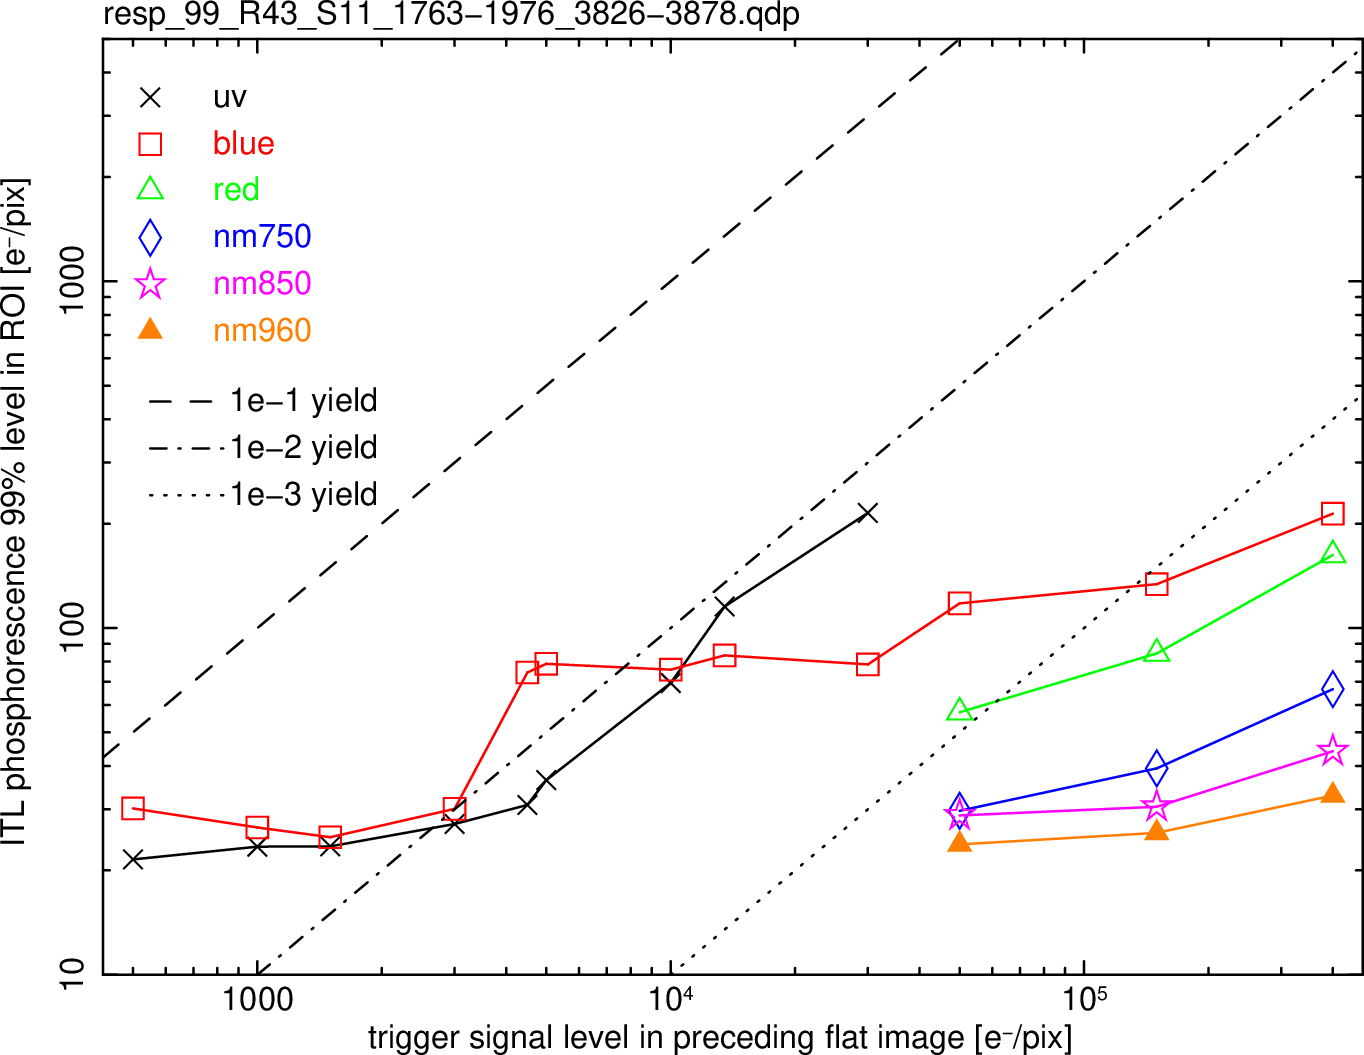
\includegraphics[width=\textwidth]{figures/phosphorescence-survey/phos_resp/resp_99_R43_S11_1763-1976_3826-3878.png}    
\end{subfigure}
\newline
\centering
\begin{subfigure}{0.45\textwidth}    
  \centering
  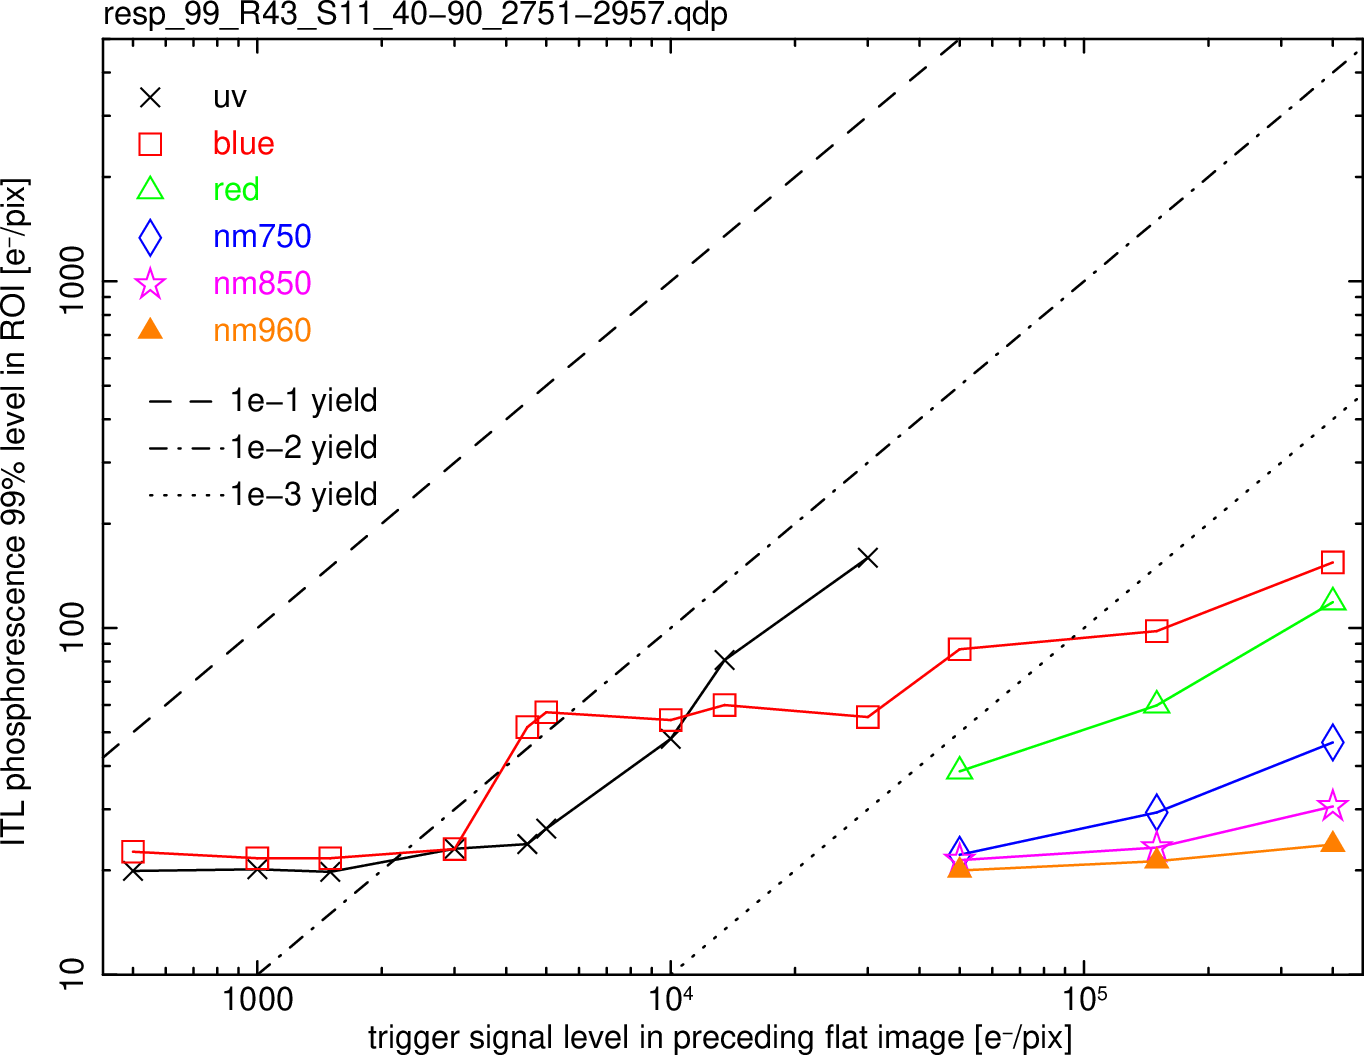
\includegraphics[width=\textwidth]{figures/phosphorescence-survey/phos_resp/resp_99_R43_S11_40-90_2751-2957.png}    
\end{subfigure}
\newline
\caption{Signal and wavelength response for phosphorescence expression (99\% level) in ROIs of images for R43\_S11. These describe bright, diffuse transient regions seen in Figs.~\ref{fig:phos:stains:R43S11} and \ref{subfig:hvb_on_R43_S11}, which apparently turn off completely when the HV Bias is {\it off}.}
\label{fig:phos:resp:R43S11}
\end{figure}

\begin{figure}[!htbp]
\centering
\begin{subfigure}{0.45\textwidth}    
  \centering
  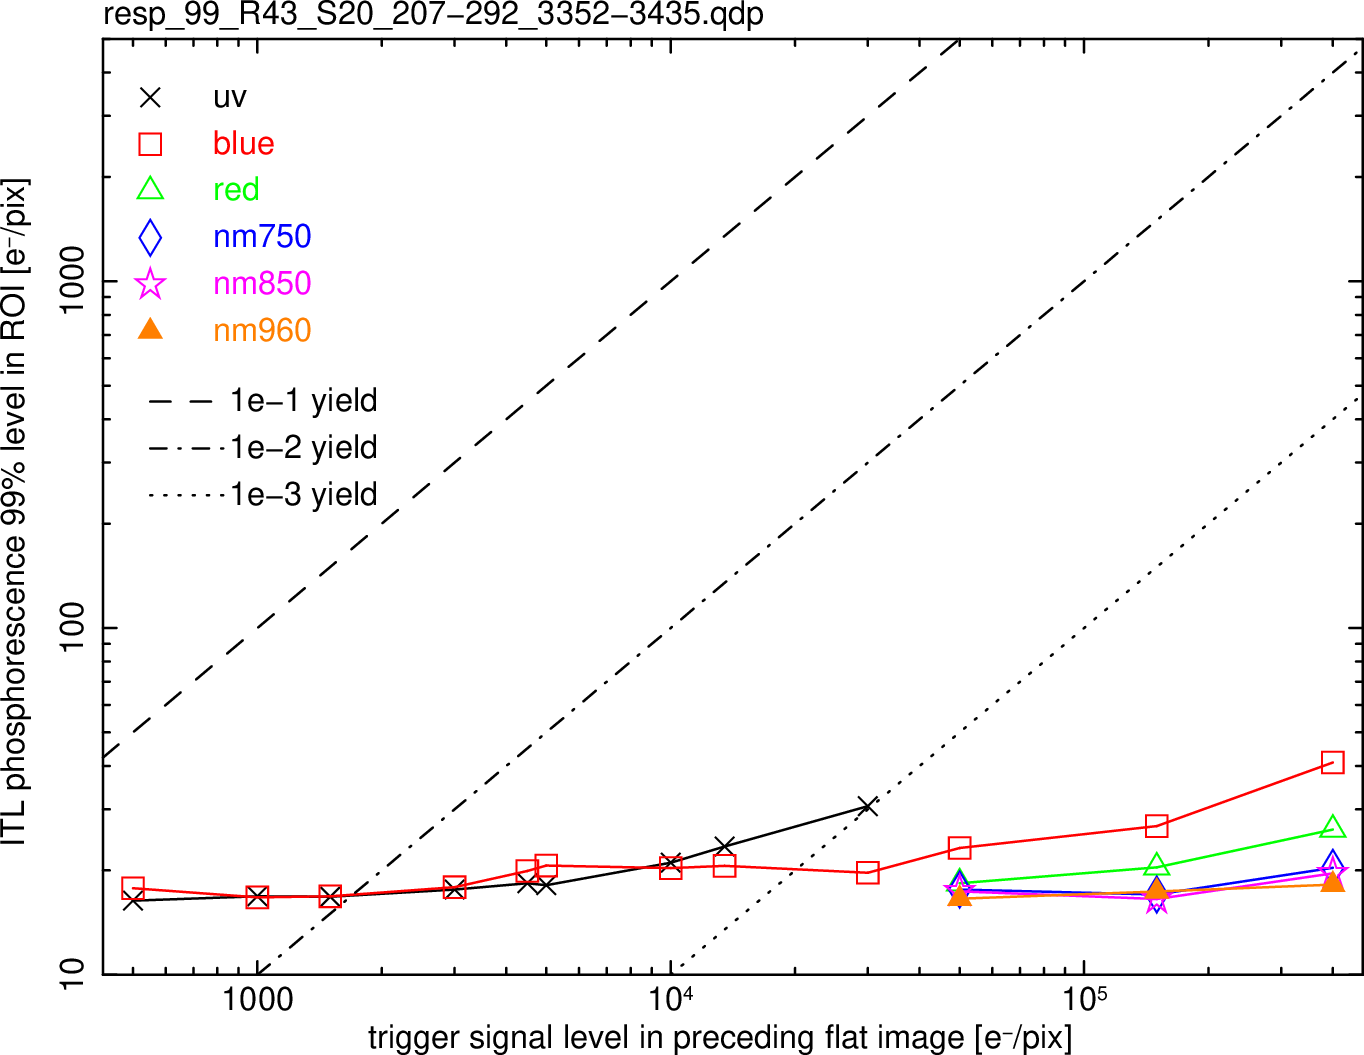
\includegraphics[width=\textwidth]{figures/phosphorescence-survey/phos_resp/resp_99_R43_S20_207-292_3352-3435.png}    
\end{subfigure}
\newline
\centering
\begin{subfigure}{0.45\textwidth}    
  \centering
  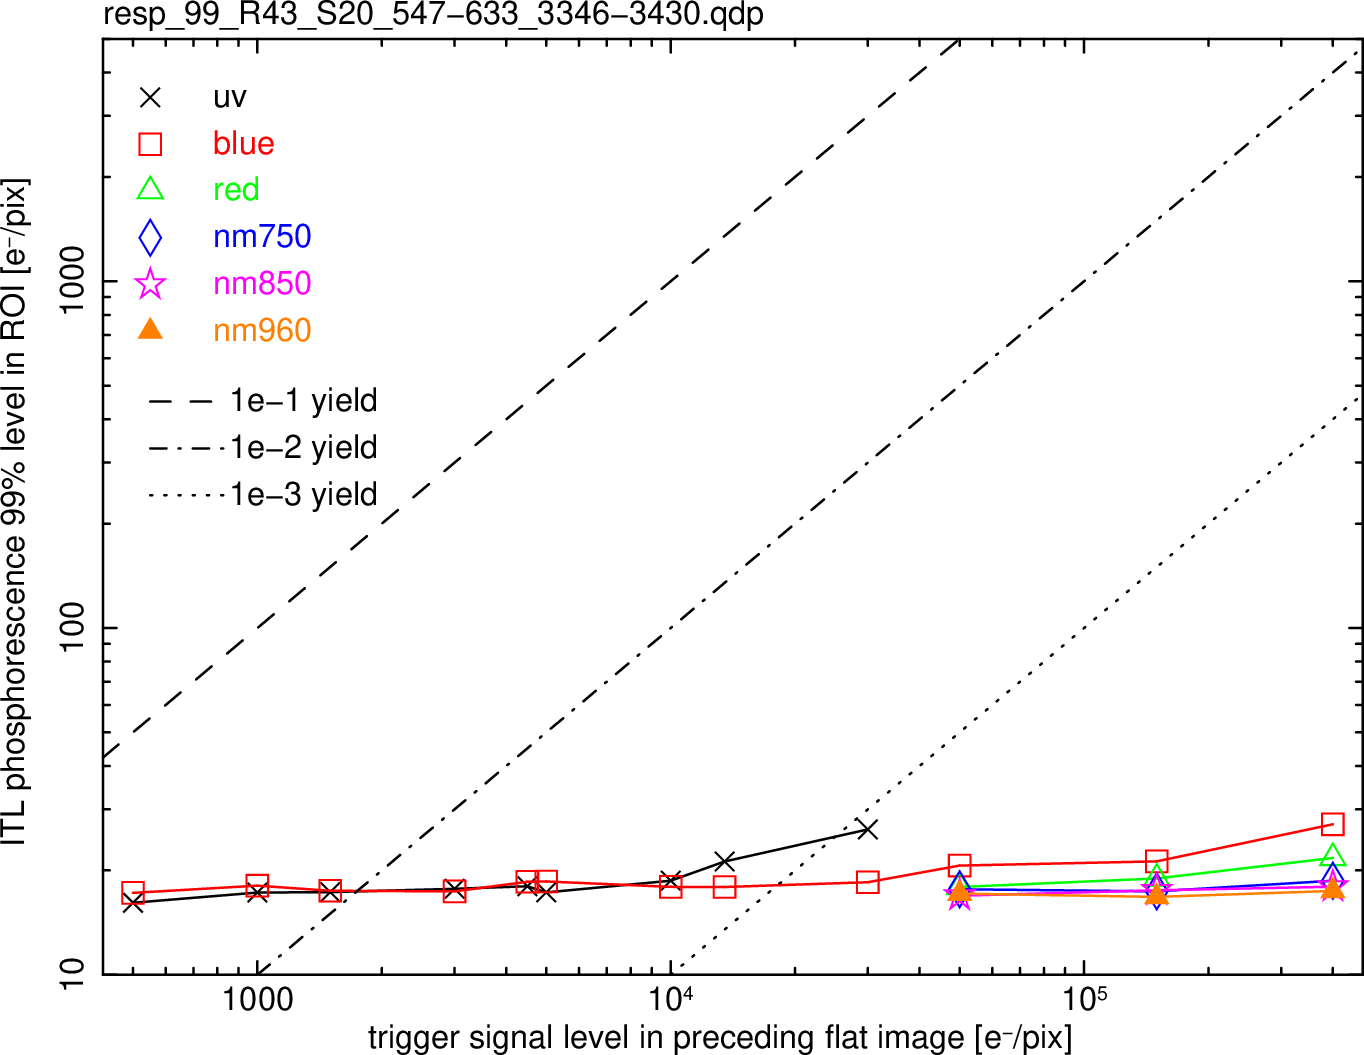
\includegraphics[width=\textwidth]{figures/phosphorescence-survey/phos_resp/resp_99_R43_S20_547-633_3346-3430.png}    
\end{subfigure}
\newline
\centering
\begin{subfigure}{0.45\textwidth}    
  \centering
  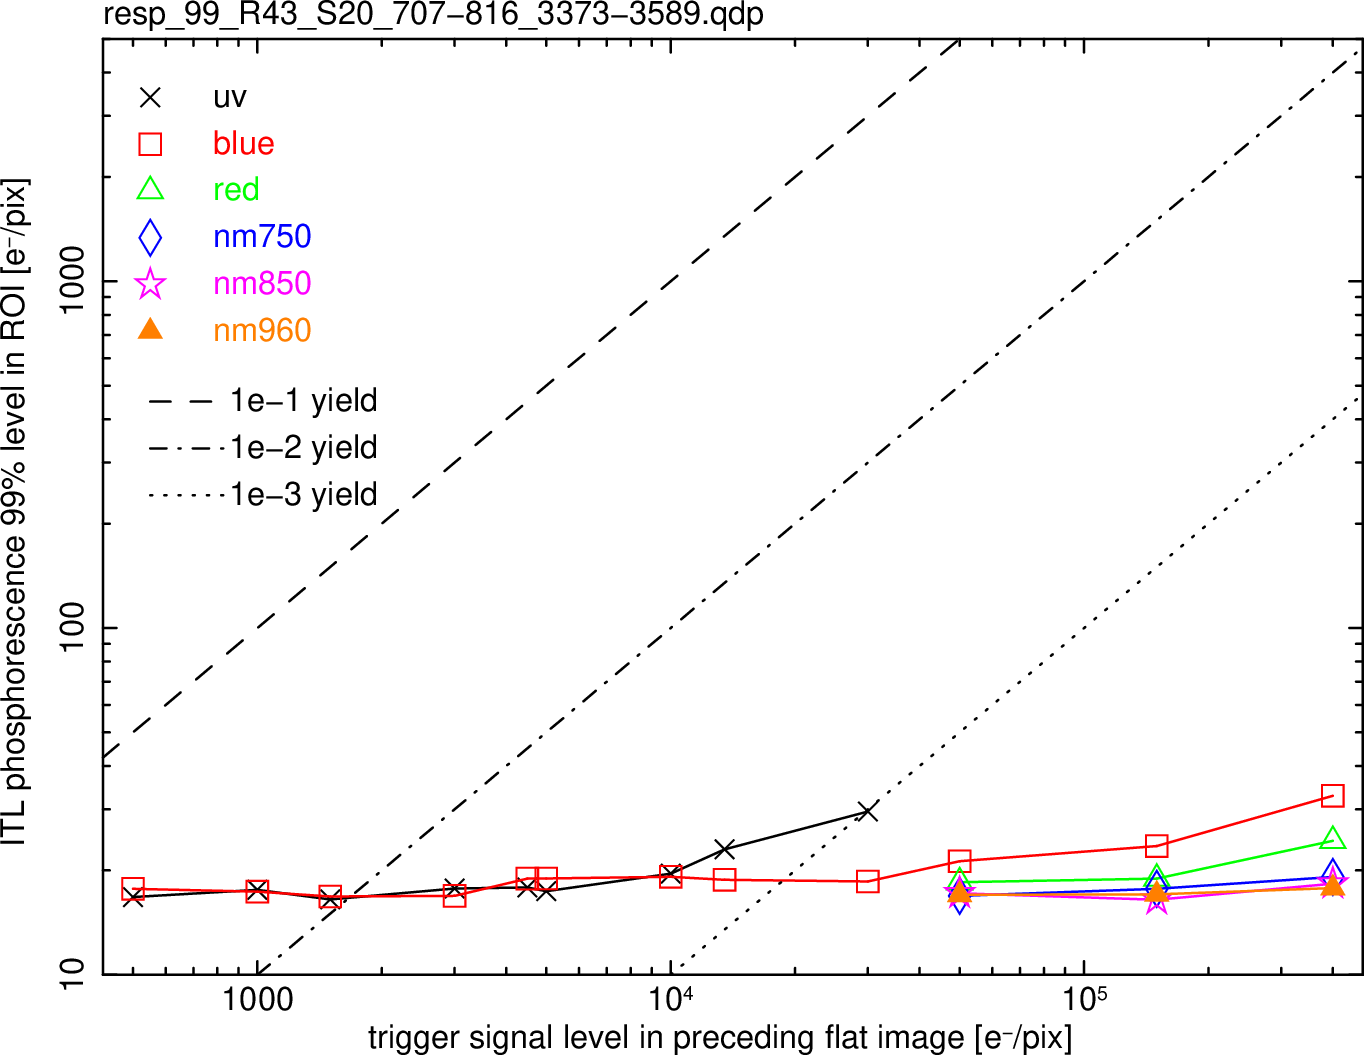
\includegraphics[width=\textwidth]{figures/phosphorescence-survey/phos_resp/resp_99_R43_S20_707-816_3373-3589.png}    
\end{subfigure}
\newline
\caption{Signal and wavelength response for phosphorescence expression (99\% level) in ROIs of images for R43\_S20. These include some of the the highly structured {\it snowflake-like} transient regions seen in Figs.~\ref{subfig:hvb_on_R43_S20} and \ref{fig:phos:stains:R43S20}.}
\label{fig:phos:resp:R43S20}
\end{figure}
